\documentclass{article}
\usepackage{xeCJK}
\usepackage{amsmath,esint,amssymb,amsthm}
\usepackage{hyperref}
\usepackage{tikz}
\usepackage{makecell}
\usepackage{multirow}
\usepackage{arcs}
\usepackage[bottom]{footmisc}
\setCJKmainfont[AutoFakeBold]{SimSun}
\usepackage{bm}
\def\v#1{\overrightarrow{#1}}
\begin{document}
\title{笔记整理}
\author{赵丰}
\maketitle
\section{草稿}
幂函数刻画的流场

针对$w(z)=Az^n,A\in \mathbb{R},n\geq \frac{1}{2}$。
若采用平面极坐标系,则流函数$\psi=Ar^n \sin n\alpha$
射线$\alpha=0,\alpha=\frac{\pi}{n}$使得$\psi=0$,因此是两条流线,若将两射线换成壁面,则其内部流场不受影响。因此
$Az^n$可以描述角域内的流动,共轭速度场为$v=nAz^{n-1}$,因此可以分$n$是否大于1讨论速度场在角点和无穷远点的零极点特性,如图
\ref{fig:powerComplexFunctionField}所示:

\begin{figure}[!ht]
 \centering
 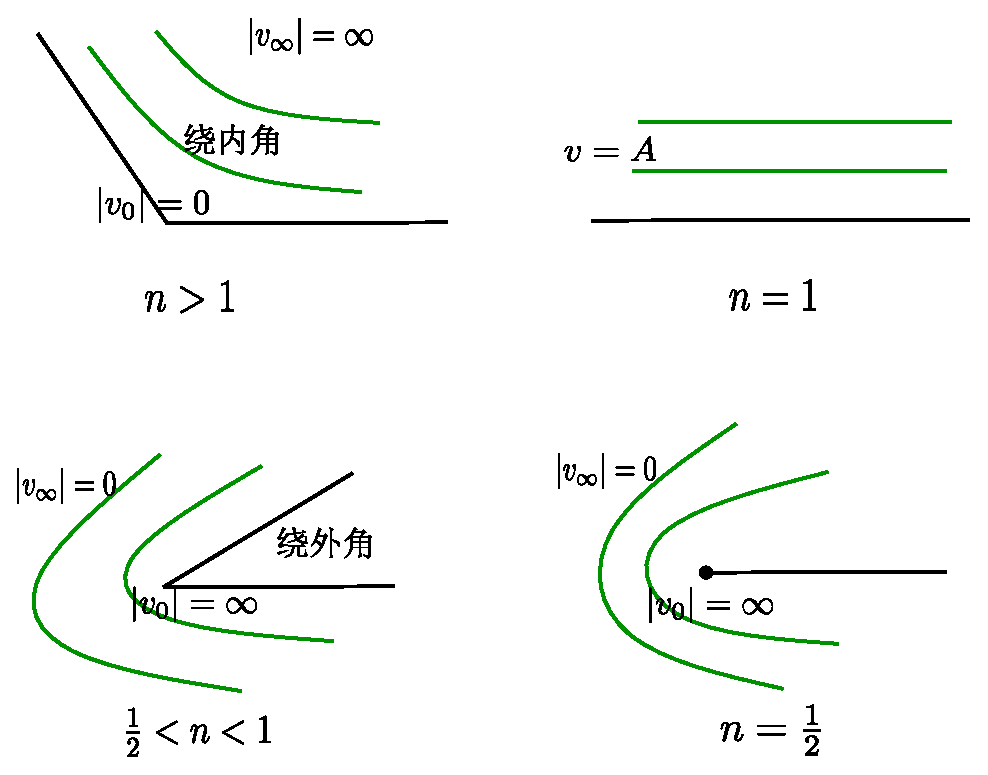
\includegraphics[width=8cm]{powerComplexFunctionField.eps}
 \caption{四类基本解等$\varphi$线和等$\psi$线的形状}\label{fig:powerComplexFunctionField}
\end{figure}

下面利用复势求解圆柱线流问题,考虑沿x轴方向的均匀来流$v_{\infty}=U$,原点处有一圆柱,在复平面内投影为一半径为$a$的圆。
复势可看成三类基本解的叠加:
\begin{equation}\label{eq:92Uk}
w(z)=Uz+\frac{k}{z}+\frac{\Gamma}{2\pi i}\ln z
\end{equation}
其中$Uz$为均匀流场,与无穷远的来流条件相匹配;
$\frac{1}{z}$为偶极子产生的流场,系数$k$待定,与壁面不可穿透条件相适应;
$\ln z$为点涡产生的流场,与流场绕任意不可缩流线的环量为$\Gamma$相适应。

由不可穿透性条件可以确定$k$的值,\eqref{eq:92Uk}式中令$z=ae^{i\alpha}$,并取虚部(流函数)为常数得:
\begin{equation}
Ua\sin\alpha-\frac{k}{a}\sin\alpha-\frac{\Gamma}{2\pi}\ln a=c
\end{equation}
由$\alpha$的任意性,得$k=Ua^2$,因此求得复势为:
\begin{equation}
w(z)=Uz+\frac{Ua^2}{z}+\frac{\Gamma}{2\pi i}\ln z
\end{equation}
取实部得速度势函数$\varphi$为:
\begin{equation}
\varphi=Ur\cos\alpha+\frac{Ua^2\cos\alpha}{r}+\frac{\Gamma \alpha}{2\pi}
\end{equation}
在极坐标下得到速度场为:
\begin{align}\notag
v_r =& \frac{\partial \varphi}{\partial r}=U(1-\frac{a^2}{r^2})\cos\alpha\\
v_{\alpha} = & \frac{1}{r}\frac{\partial \varphi}{\partial \alpha}=-U(1+\frac{a^2}{r^2})\sin\alpha+\frac{\Gamma}{2\pi r}
\end{align}
若考虑壁面的速度场分布,$r=a$因此$v_r=0$。

当$\Gamma=0$即流场速度环量为零时,类似\ref{sec:81}小节讨论的关于圆球绕流问题,在来流方向
的前后驻点处($\alpha=0,\pi$)速度为零,压强最大。对于壁面$\alpha$角位置的压强,由Bernoulli方程可求出$p=p_{\infty}+\frac{1}{2}\rho U^2 (1-4\sin^2\alpha)$

当$\Gamma\neq 0$时(通常由圆柱自身转动引起周围流体的环量),壁面不一定有驻点。若驻点存在,则适合方程$\frac{d w}{d z}=0$,即为下面复二次方程的根:
\begin{equation}
2\pi i U z^2 + \Gamma z - 2\pi i U a^2=0
\end{equation}
其通解为:
\begin{equation}
z=\frac{-\Gamma\pm \sqrt{\Gamma^2-16\pi^2U^2a^2}}{4\pi i U}
\end{equation}
若$|\Gamma|>4\pi Ua$,则方程的两根都在虚轴上,由于其乘积为$-a^2$,所以有一根在壁面内,舍去。若$\Gamma<0$,则速度场有一个驻
出现在虚轴的负半轴壁面外的地方。

若$|\Gamma|=4\pi Ua$,两根重合,同样考虑$\Gamma<0$,这时驻点为$z=-ia$

若$|\Gamma|<4\pi Ua$,计算两根的模均为$a$,因此两驻点均在壁面上,当$\Gamma<0$时,两驻点虚部为负,关于虚轴对称。

同理可得$\Gamma\neq 0$时壁面压力场为:
\begin{equation}
p=p_{\infty}+\frac{1}{2}\rho(U^2-(-2U\sin\alpha+\frac{\Gamma}{2\pi a})^2)
\end{equation}

计算流体对壁面的合力为:
\begin{equation}
\v{F}=-\int_{0}^{2\pi} p\v{n}d\alpha
\end{equation}
化为分量形式得$F_x=0,F_y=-\int_{0}^{2\pi} pa\sin\alpha d\alpha=-\rho U \Gamma$,当$\Gamma<0$时$F_y>0$,即对于顺时针的环量可以产生升力。
此即儒科夫斯基升力定理。
\begin{equation}
\end{equation}

\begin{thebibliography}{99}
\bibitem{mixedProduct} \href{https://en.wikipedia.org/wiki/Triple_product}{https://en.wikipedia.org/wiki/Triple\_product}
\bibitem{velocityGradient}\href{http://www.continuummechanics.org/velocitygradient.html}{http://www.continuummechanics.org/velocitygradient.html}
\bibitem{angularVelocityTensor}\href{https://en.wikipedia.org/wiki/Angular_velocity#Angular_velocity_tensor}{https://en.wikipedia.org/wiki/Angular\_velocity\#Angular\_velocity\_tensor}
\bibitem{CylindricalCoordinates}\href{https://en.wikipedia.org/wiki/Divergence#Cylindrical_coordinates}{https://en.wikipedia.org/wiki/Divergence\#Cylindrical\_coordinates}
\bibitem{CurlFormular}\href{https://en.wikipedia.org/wiki/Curl_(mathematics)}{https://en.wikipedia.org/wiki/Curl\_(mathematics)}
\bibitem{FundamentalSolution}\href{https://en.wikipedia.org/wiki/Fundamental_solution}{https://en.wikipedia.org/wiki/Fundamental\_solution}
\bibitem{GreenFunction}\href{https://en.wikipedia.org/wiki/Green\%27s_function#Green.27s_functions_for_the_Laplacian}{https://en.wikipedia.org/wiki/Green\%27s\_function\#Green.27s\_functions\_for\_the\_Laplacian}
\bibitem{Del}\href{https://en.wikipedia.org/wiki/Del_in_cylindrical_and_spherical_coordinates}{https://en.wikipedia.org/wiki/Del\_in\_cylindrical\_and\_spherical\_coordinates}
\bibitem{CEEquation}\href{https://en.wikipedia.org/wiki/Cauchy\%E2\%80\%93Euler_equation}{https://en.wikipedia.org/wiki/Cauchy\%E2\%80\%93Euler\_equation}
\end{thebibliography}
\end{document}